\section*{Décompte final} \label{sec:comptagePoints}
\addcontentsline{toc}{section}{Décompte final}
À la fin de la partie, deux éléments rapportent des points:
\begin{enumerate}
\item les obstacles heurtés pendant la partie
\item les cartes jouées
\end{enumerate}

\subsection*{Les points d'obstacles} \label{sec:pointsObstacles}
\addcontentsline{toc}{subsection}{Les points d'obstacles}
Pour chaque catégorie d'obstacle (\arbre, \tronc,\rocher), marquez \textbf{le nombre d'obstacle multiplié par la value du \marqueurObstacle associé}.

\begin{figure}[h]
\begin{tcolorbox}[colback=white,colframe=OliveGreen!75!black,title=Exemple]
{    \begin{multicols}{2}
    Dans cet exemple, le joueur \eau a heurté:
	\begin{itemize}
	\item \textbf{5 \arbre}
	\item \textbf{8 \tronc}
	\item \textbf{4 \rocher}
	\end{itemize}
	D'après la positions des \marqueursObstacles,
	\begin{itemize}
	\item les \tronc comptent \textbf{zéro fois}
	\item les \arbre comptent \textbf{une fois}
	\item les \rocher comptent \textbf{deux fois}
	\end{itemize}
	Le joueur \eau marque donc $8*0+5*1+4*2 = \textbf{13 points}$
    
    \columnbreak
	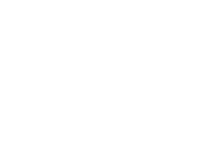
\includegraphics[scale=0.3]{regle/exemple_comptagePointsObstacle}
    \caption{Un exemple de comptage d'obstacle}
    \end{multicols}
}
\end{tcolorbox}
\end{figure}
\FloatBarrier


\subsection*{Les points de cartes} \label{sec:pointsCarte}
\addcontentsline{toc}{subsection}{Les points de cartes}
